\documentclass[12pt,a4paper]{article}

\usepackage{graphicx,amsmath,amssymb,float,caption,hyperref,fancyhdr}
\usepackage{newtxtext,newtxmath}
\usepackage{geometry,booktabs,tabularx,array,longtable,microtype}
\usepackage{xcolor}
\usepackage{tikz}
\usetikzlibrary{arrows.meta,positioning,calc}
\geometry{margin=1in}
\setlength{\headheight}{14.5pt}
\pagestyle{fancy}
\fancyhf{}
\lhead{NE39  SG31 + Nine IBR  reclose}
\rhead{\thepage}
\renewcommand{\headrulewidth}{0.4pt}
\renewcommand{\arraystretch}{1.12}
\emergencystretch=1.5em
\hypersetup{colorlinks=true,linkcolor=blue!45!black,citecolor=blue!45!black,
  urlcolor=blue!45!black}

\DeclareMathOperator{\clamp}{clamp}
\DeclareMathOperator{\sat}{sat}
\newcommand{\pu}{\ifmmode\,\mathrm{p.u.}\else\ p.u.\fi}
\newcommand{\second}{\ifmmode\,\mathrm{s}\else\ s\fi}
\newcommand{\vect}[1]{\boldsymbol{#1}}

% Graphics search path (report lives in docs/source/).
\graphicspath{{figures/}{figures/ne39_160s_reclose_cpp/}}
\newcommand{\datadir}{figures/ne39_160s_reclose_cpp}
\newcommand{\code}[1]{\texttt{\detokenize{#1}}}

\usepackage{pgfplots,pgfplotstable}
\pgfplotsset{compat=1.18}

% Graphics search path (report lives in docs/source/).
\graphicspath{{figures/}{figures/ne39_160s_reclose_cpp/}}

\definecolor{pgreen}{RGB}{41,153,69}
\definecolor{pred}{RGB}{191,45,45}
\definecolor{pblue}{RGB}{46,107,191}
\definecolor{pyellow}{RGB}{199,178,38}
\definecolor{pgrey}{RGB}{90,90,90}

\title{\textbf{NE39 True-Trip SG31 Reclose Study: Supervisor-Driven Restoration
(C++ Engine Edition)}\\
\large One Classical Reclose SG (six state) and Nine 17-State Dual-mode-IBR Converters\\[1mm]
\normalsize Power Flow, Equilibrium, Fault Cycle Events, and 160-s Time-Domain Simulation}
\author{In-house Power-Flow Project}
\date{16 October 2026}

\begin{document}
\maketitle

\begin{abstract}
This report documents the NE39 (New England IEEE 39-bus) mixed-resource chronology
studied by the project, as produced by the \code{GridFormLab C++ stage2-ibr}
engine.  Thirty-nine buses carry one synchronous machine at bus~31
(SG31, a six-state sixth-order reclose plant with its terminal estimator) and
nine Dual-mode-IBR converters
(IBR30, IBR32--IBR39) at buses 30 and 32--39, initialised in grid-forming (GFM)
mode under an amplitude--frequency severity supervisor.
The reported products share one accepted equilibrium: case input tables, solved bus
voltages, branch flows, device injections, an event-fence 160-second time-domain
simulation (SG trip at 20~s, bus-16 fault $Z_f=j0.1$~pu at 60--60.15~s, reclose
request at 100~s), and the observed guard-driven SG reclose at 100.499~s.
The simulation is a fixed-step implicit trapezoidal integration at
$h=1$~ms with a coupled Newton solve (160{,}000 accepted steps, no rejections).
Plots are rendered from CSV evidence exported from the C++ run artifact and
re-rendered at the report typography.  This edition quotes C++ numbers
exclusively: the reclose instant differs from the MATLAB edition (119.55~s)
because the two engines run different synchronism-guard policies, and every
difference between the editions is itemised in the closing data-provenance
table.  Quantities the C++ recorder does not export (per-event KCL residuals,
transition-trial evidence, excursion flags) are marked not-exported in place
instead of being copied from the other edition.
\end{abstract}

\newpage
\tableofcontents
\newpage

\section{Scope, sources and reproduction}\label{sec:scope}

The study system is the TAMU New England 39-bus network with one modelled SG at
the slack bus and nine modelled IBRs at buses 30, 32--39.  The whole system is
assembled as a single all-KCL composite differential--algebraic system in which
the SG and every IBR contribute their own differential state block and their own
injection; no device is delegated to an external solver, model, or reference
program.

\paragraph{Chronology.}
The scheduled disturbance times are case-defined constants; the reclose instant
is an outcome read from the accepted event log.  Section~\ref{sec:chrono} shows
the four operating periods and the transition instants.

\paragraph{Figure source and no-synthetic-signal contract.}
The transient figures (Section~\ref{sec:transient}) are rendered from the
accepted trajectory of the C++ run artifact
\code{stage2\_smoke\_ne39\_008\_gfm160s\_golden} (160{,}000 accepted rows at
1~kHz).  The per-device series are reconstructed from the recorded bus voltages
and angles through the case network by bus KCL (the load is folded at the
equilibrium voltage; the reconstruction and its validation are itemised in the
closing provenance table) and are plotted at every 10th sample (16{,}001 rows)
--- display decimation only, disclosed here and in the captions; every quoted
number is computed on the full record.  Nothing is smoothed, filtered, clipped,
offset, interpolated, or augmented with synthetic noise.  Every number in this
report is read from the C++ run artifact or computed from the case it consumed;
no gate is relaxed and no simulation is re-run.

\paragraph{Classification.}
The SG AC/flux equations and the IBR AC/control equations are
\textsf{SOURCE\_MAPPED} or \textsf{PROJECT\_DERIVED} as labelled where they first
appear; machine and converter parameters, per-unit bases, and the disturbance
times are \textsf{CASE\_DEFINED}; the predictor and step-subdivision policy are
\textsf{NUMERICAL\_METHOD}.  The run classification (\code{run\_kind=SMOKE}) is
carried from the C++ manifest and is not re-decided here.

%=============================================================================
\section{Disturbance chronology}\label{sec:chrono}
%=============================================================================
The scheduled disturbance times are \textsf{CASE\_DEFINED} constants of the
event structure; the reclose instant is an outcome read from the accepted event
log.  Figure~\ref{fig:periods} shows the six operating periods and the
transition instants.  The bus-16 fault is applied at $t=60.000\second$ and
cleared at $t=60.150\second$ (a $0.150$\second fault, impedance
$Z_f=j0.1\pu$); the reclose request is armed at $t=100\second$ and the SG31
close is committed at $t=100.499\second$ (an offline age of $80.499$\second
against the declared $0.5$\second minimum).

\begin{figure}[H]
\centering
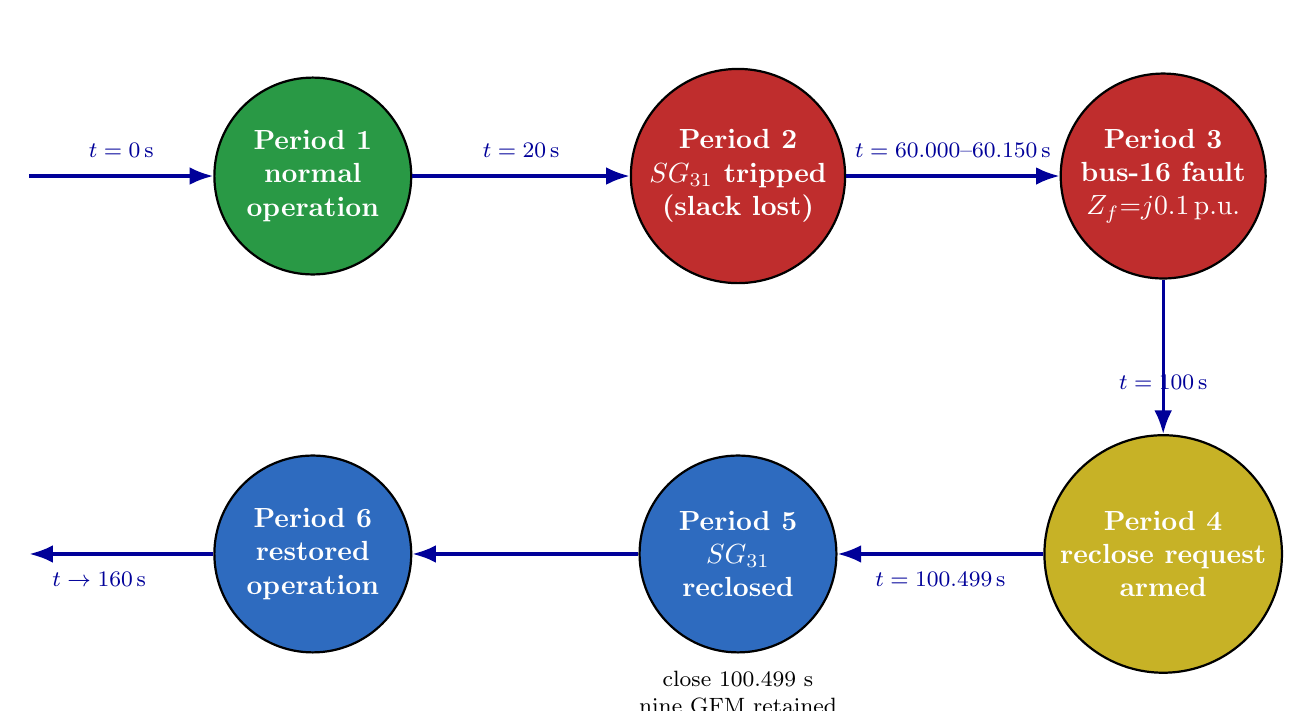
\begin{tikzpicture}[
  font=\normalsize,
  per/.style={circle,draw,thick,minimum size=2.5cm,inner sep=2pt,
    align=center,text=white,font=\bfseries},
  tlab/.style={midway,above=1mm,font=\footnotesize},
  tlabb/.style={midway,below=1mm,font=\footnotesize},
  arr/.style={-{Latex[length=3mm]},very thick,color=blue!60!black}]

\node[per,fill=pgreen] (p1) at (0,0)     {Period 1\\ normal\\ operation};
\node[per,fill=pred]   (p2) at (5.4,0)   {Period 2\\ $SG_{31}$ tripped\\ (slack lost)};
\node[per,fill=pred]   (p3) at (10.8,0)  {Period 3\\ bus-16 fault\\ $Z_f{=}j0.1\pu$};
\node[per,fill=pyellow](p4) at (10.8,-4.8){Period 4\\ reclose request\\ armed};
\node[per,fill=pblue]  (p5) at (5.4,-4.8){Period 5\\ $SG_{31}$\\ reclosed};
\node[per,fill=pblue]  (p6) at (0,-4.8)  {Period 6\\ restored\\ operation};

\draw[arr] (-3.6,0) -- node[tlab]{$t=0\second$} (p1);
\draw[arr] (p1) -- node[tlab]{$t=20\second$} (p2);
\draw[arr] (p2) -- node[tlab]{$t=60.000$--$60.150\second$} (p3);
\draw[arr] (p3) -- node[tlabb]{$t=100\second$} (p4);
\draw[arr] (p4) -- node[tlabb]{$t=100.499\second$} (p5);
\draw[arr] (p5) -- (p6);
\draw[arr] (p6) -- node[tlabb,pos=0.62]{$t\to160\second$} ++(-3.6,0);

\node[font=\footnotesize,below=3pt of p5,align=center,text=black]
  {close $100.499$\second\\ nine GFM retained};
\end{tikzpicture}
\caption{Six-period disturbance chronology.  Green: undisturbed.  Red: a
contingency that removes the SG slack or faults a bus.  Yellow: the armed
reclose request.  Blue: the restorative reclose and the restored operation.
Scheduled instants ($0$, $20$, $60.000$--$60.150$, $100\second$) are
case-defined; the reclose instant ($100.499\second$) is read from the C++
guard record \code{guard\_reclose.json}.}
\label{fig:periods}
\end{figure}

The products in this report are deliberately separated:
\begin{enumerate}
  \item case inputs (bus dispatch schedules, branch impedances) and the accepted
        initial equilibrium (SG31 synchronous and all nine IBRs GFM);
  \item the 160-\second{} event chronology with automatic GFM switching armed and a
        supervisor-driven SG31 release;
  \item the observed reclose transaction and the final mode inventory.
\end{enumerate}

\subsection{Honest status of this run}
\begin{itemize}
\item The run integrated the full horizon to $t=160$~s on the fixed-step
      implicit trapezoidal stepper at $h=1$~ms: 160{,}000 attempted and
      160{,}000 accepted steps, 0 failed, 300{,}126 coupled-Newton iterations
      and 300{,}126 Jacobian evaluations (335.6~s wall time).
\item The SG reclose transaction is the guard-driven close at $t=100.499$~s
      (\code{guard\_reclose.json}; the \code{sg\_on} event at $t=100.000$~s
      armed the guard): margins at the commit are $dV=1.73\times10^{-14}$~pu,
      $df=5.09\times10^{-5}$~pu, $d\theta=4.398^\circ$ against the recorded
      frozen thresholds $0.05$~pu, $0.001$~pu, $10^\circ$, and the offline age
      is 80.499~s against the declared 0.5-s minimum.
\item The C++ recorder exports no per-event KCL residuals and no
      transition-trial evidence: the trip-point forward transition trial of the
      MATLAB edition is \emph{not computable} from this artifact and is
      reported as not-exported rather than copied
      (Table~\ref{tab:events}).
\item The recorded trajectory is 160{,}000 rows at 1~kHz
      ($t=0.001$--$160.000$~s) with the bus angles stored in radians (converted
      to degrees for the report); the export carries no voltage-excursion flag
      column and no step-rejection record (the fixed-step stepper rejected no
      step).
\item Per-device series in this report are reconstructed by bus KCL from the
      recorded voltages and the case network; at the equilibrium the
      reconstruction agrees with the aligned $dq$ identity of the stored
      converter currents to $3.35\times10^{-7}$~pu ($P$) and
      $8.2\times10^{-8}$~pu ($Q$) --- the reconstruction route and its
      transient limitations are itemised in the closing provenance table.
\end{itemize}

\section{Automatic GFL/GFM selection: the severity index}\label{sec:sev}

Each IBR carries a two-state supervisor that decides whether it should behave
as a grid-following current source (GFL) or as a grid-forming voltage source
(GFM).  The decision is driven by a scalar severity $S(t)\in[0,1]$ built from
normalised sub-indices: a voltage-deviation index $J_V$ and a
frequency-deviation index $J_f$, optionally extended by rate-of-change
sub-indices.

\paragraph{Sub-indices.}
Let $|V_i(t)|$ be the terminal voltage magnitude of IBR~$i$ and $V_i^{\star}$
the healthy per-bus power-flow magnitude at the SG-online operating point
(Section~\ref{sec:pf}).  Let $f_{\rm coi}(t)$ be the centre-of-inertia
frequency, weighted by each online device's system inertia.  With bases
$\Delta V_{\rm base}=0.10\pu$ and $\Delta f_{\rm base}=0.50$~Hz,
\begin{equation}
  J_V(t)=\frac{\bigl|\,|V_i(t)|-V_i^{\star}\,\bigr|}{\Delta V_{\rm base}},
  \qquad
  J_f(t)=\frac{\bigl|\,f_{\rm coi}(t)-f_0\,\bigr|}{\Delta f_{\rm base}},
  \qquad f_0=60~\mathrm{Hz}.
  \label{eq:jvjf}
\end{equation}

\paragraph{Two-term severity (AGSI).}
The reported severity is the saturated equal-weight average
\begin{equation}
  S(t)=\sat_{[0,1]}\!\Bigl(\tfrac12 J_V(t)+\tfrac12 J_f(t)\Bigr),
  \qquad
  \sat_{[0,1]}(z)=\min\{1,\max\{0,z\}\}.
  \label{eq:agsi}
\end{equation}
$J_V$ responds to a local voltage collapse or overshoot; $J_f$ responds to a
system-wide frequency excursion such as the one that follows the loss of the
SG slack at $t=20$~s.  The equal weighting is a \textsf{PROJECT\_DERIVED}
choice and is frozen before any result is read.

\paragraph{Four-term weighted variant (opt-in).}
The study design also defines an opt-in extension with device-local rate
sub-indices.  With device-local frequency $f_i(t)$, ROCOF
$\dot f_i(t)$, and ROCOV $\dot\nu_i(t)$, and bases
$[\Delta V_{\rm base},\Delta f_{\rm base},\Delta r_{f},\Delta r_{\nu}]
=[0.10\pu,\,0.50~\mathrm{Hz},\,1~\mathrm{Hz/s},\,1~\mathrm{pu/s}]$,
\begin{equation}
\begin{aligned}
  J_{\dot f}(t)&=\frac{|\dot f_i(t)|}{\Delta r_{f}},&
  J_{\dot\nu}(t)&=\frac{|\dot\nu_i(t)|}{\Delta r_{\nu}},\\
  S_{w}(t)&=\sat_{[0,1]}\!\bigl(
      0.35\,J_V+0.35\,J_f+0.15\,J_{\dot f}+0.15\,J_{\dot\nu}\bigr).&&
\end{aligned}
\label{eq:weighted}
\end{equation}
The weights $[0.35,0.35,0.15,0.15]$ and the bases above are
\textsf{PROJECT\_DERIVED, UNVALIDATED} study design: the weighted variant is
armed only when explicitly enabled, and omission keeps the two-term
COI scalar~\eqref{eq:agsi} in force unchanged.  The weights and bases are
validated at option resolution (nonnegative, weights sum to one, positive
bases), and the healthy-PF reference must match each device's bus uniquely ---
otherwise the weighted sample is refused as invalid evidence, never silently
given a guessed reference.

\paragraph{Why $[0.35,0.35,0.15,0.15]$.}
The voltage and frequency deviations $J_V,J_f$ are the two quantities the
supervisor can trust at every instant: each is normalised by a declared base
($\Delta V_{\rm base}=0.10$~pu, $\Delta f_{\rm base}=0.50$~Hz) taken from the
same study design, so they enter the severity with equal standing and share
$0.35+0.35=0.70$ of the total weight.  The rate sub-indices $J_{\dot f},
J_{\dot\nu}$ are supporting evidence only: their bases ($1$~Hz/s, $1$~pu/s)
are design orders of magnitude rather than Measured envelopes, their raw
signals are noisier (finite-difference of the accepted samples), and neither
corresponds to a gate the supervisor owns.  They therefore carry the remaining
$0.15+0.15=0.30$, enough to sharpen the trigger during fast transients without
ever outweighing the two primary deviations.  The split is a
\textsf{PROJECT\_DERIVED} study choice -- 70/30 between level and rate
information -- frozen before any result was read, and it is not a certified
or grid-code weighting.

\paragraph{Hysteresis, dwell, and the gates the index does not replace.}
A bare threshold on $S$ would chatter.  The supervisor therefore uses an
asymmetric two-level comparator with minimum dwell times,
\begin{equation}
  \begin{aligned}
    \text{GFL}\to\text{GFM}:&\quad S\ge\Gamma_{\rm on}=0.65
       \ \text{held for}\ T_{d,\rm on}=0.10\second,\\
    \text{GFM}\to\text{GFL}:&\quad S\le\Gamma_{\rm off}=0.35
       \ \text{held for}\ T_{d,\rm off}=1.00\second.
  \end{aligned}
  \label{eq:hyst}
\end{equation}
The gap $\Gamma_{\rm on}>\Gamma_{\rm off}$ is the hysteresis band.  A separate
reference-loss guard forces every online IBR to GFM the instant the SG slack
is lost, before the dwell logic runs, so the network never spends a step
without a voltage reference.  Thresholds and dwell times resolve as one
contract: when the same scalar is supplied through two spellings and they
disagree, the run fails closed instead of picking one.  The severity index
arms and holds converters, but it never gates the SG reclose itself --- the
SG close is a strict transactional commit (synchronism triple, dwell, and
physical KCL at the replaced rows, all passing at the same instant), and the
diagnostic SCR of Section~\ref{sec:transient} never enters them either.

\section{Case data and index maps}

\subsection{System and resource map}

The network is the 100-MVA, 60-Hz TAMU New England 39-bus data set.  The
source archive is transcribed with SHA-256 recorded in the case struct; the
project adds the composition, the Slack point SG31 at its case design
setpoint $V=1.0778$~pu, and the converter ratings.  The mixed resource map is
\begin{center}\footnotesize
\begin{tabular}{ccllc}
\toprule
Device index & Bus ID & Device & Model & Initial mode\\
\midrule
1 & 31 & SG31 & \code{sg_classical_reclose} (6 states) & synchronous\\
2--10 & 30, 32--39 & IBR30, 32--39 & \code{Dual-mode-IBR} (17 states) & GFM\\
\midrule
\multicolumn{4}{r}{Runtime dynamic inventory} & \multicolumn{1}{c}{$7+9(17)=160$}\\
\bottomrule
\end{tabular}
\end{center}
The C++ stage2 state vector carries the SG31 plant's six states plus the
terminal-estimator speed state $\hat\nu$ (the estimator angle $\hat\theta$ is
shared with the plant), so the runtime dynamic count is $7+9(17)=160$ states
alongside 78 algebraic voltages.

\paragraph{IBR parameters at each bus.}  All nine converters share the
Dual-mode-IBR plant constants ($L_f=0.15$~pu, $R_f=0.015$~pu,
$C_{dc}=0.0237216$~pu, $V_{dc,\rm ref}=1$~pu, $M=3.3209$~s,
$D_v=33.2095$~pu, $\tau_E=0.4$~s, $k_Q=0.2$, $k_E=8$, $k_{pV}=1.2$,
$k_{iV}=3.2587$; GFL PLL $k_p=1.2$, $k_i=5$) and differ only in their port
rating and duty:
\begin{center}\footnotesize
\begin{tabular}{crrrrrr}
\toprule
Device & Bus & $S_{\rm rating}$ pu & $P_{\rm max}$ pu & $Q_{\rm max}$ pu & Schedule $P$ pu & Schedule $Q$ pu\\
\midrule
IBR30 & 30 & 44.000 & 4.300  & 39.300 & 2.500  & ---\\
IBR32 & 32 & 44.400 & 11.200 & 38.300 & 6.500  & ---\\
IBR33 & 33 & 36.700 & 10.900 & 31.100 & 6.320  & ---\\
IBR34 & 34 & 11.800 & 8.800  & 5.900  & 5.080  & ---\\
IBR35 & 35 & 43.500 & 11.200 & 37.500 & 6.500  & ---\\
IBR36 & 36 & 35.300 & 9.700  & 30.200 & 5.600  & ---\\
IBR37 & 37 & 18.200 & 9.300  & 13.400 & 5.400  & ---\\
IBR38 & 38 & 35.300 & 14.300 & 28.300 & 8.300  & ---\\
IBR39 & 39 & 33.100 & 17.200 & 24.300 & 10.000 & ---\\
\midrule
\multicolumn{6}{r}{Total converter schedule $P$} & \multicolumn{1}{c}{56.200}\\
\bottomrule
\end{tabular}
\end{center}
(The same values in MW/MVAr on the 100-MVA base: $S_{\rm rating}$
4400/4440/3670/1180/4350/3530/1820/3530/3310~MVA, schedule $P$
250/650/632/508/650/560/540/830/1000~MW for IBR30, 32--39.)
The P schedule is the rating-proportional dispatch of the composition
contract; the reactive duty is NOT a converter schedule --- each IBR bus
carries the fixed port reactor of the chronology design
($B_s=-Q_r/S_{base}$, $\sum Q_r = 161.68$~pu), so the converter absorbs
the reactor's demand through its Q--V loop at the solved voltage.  Current
limits are $I_{max}^{SS}=I_{max}^{F}=1.2\pu$ device base with
$E_{\rm max}=1.2$, $E_{\rm min}=0.8\pu$, and the fault contract is balanced
positive-sequence RMS with GFM current circles.

Algebraic voltage order is
\[
\vect y=[V_{x,1},V_{y,1},V_{x,2},V_{y,2},\ldots,V_{x,39},V_{y,39}]^{\mathsf T},
\qquad V_k=V_{x,k}+jV_{y,k},
\]
78 algebraic variables for 39 buses.  SG bus types on the source RAW are
PVGEN/slack-derived by the project composition: bus~31 is the declared slack
($V=1$~pu, $0^\circ$), the remaining source-generator buses (32, 35, 38, 39)
are PV in the source PF but this composition converts every non-SG31 machine
to a converter terminal, and the nine IBR buses are effective PQ in the
equilibrium solve.

\subsection{Bus input data}

\begin{table}[H]\centering\footnotesize
\caption{Case bus data.  These are inputs, not solved PF results: the load
schedules $P_d$/$Q_d$ and shunt admittances $G_s$/$B_s$ straight from the
composition, per unit on the 100-MVA base.}
\pgfplotstabletypeset[col sep=comma,
 columns={bus_id,type,Pd_pu,Qd_pu,Gs_pu,Bs_pu},
 columns/bus_id/.style={column name=Bus},columns/type/.style={column name=Role,string type},
 columns/Pd_pu/.style={column name=$P_L$ pu,fixed,fixed zerofill,precision=3},
 columns/Qd_pu/.style={column name=$Q_L$ pu,fixed,fixed zerofill,precision=3},
 columns/Gs_pu/.style={column name=$G_s$ pu,fixed,fixed zerofill,precision=3},
 columns/Bs_pu/.style={column name=$B_s$ pu,fixed,fixed zerofill,precision=3},
 every head row/.style={before row=\toprule,after row=\midrule},every last row/.style={after row=\bottomrule}]
{\datadir/case_bus_data.csv}
\end{table}

\begin{table}[H]\centering\footnotesize
\caption{Case branch series and charging data in source row order (46 branches,
per unit on the 100-MVA base).}
\pgfplotstabletypeset[col sep=comma,
 columns={branch_index,from_bus,to_bus,r_pu,x_pu,b_pu},
 columns/branch_index/.style={column name=Index},columns/from_bus/.style={column name=From},
 columns/to_bus/.style={column name=To},columns/r_pu/.style={column name=$r$ pu},
 columns/x_pu/.style={column name=$x$ pu},columns/b_pu/.style={column name=$b_c$ pu},
 columns/r_pu/.append style={fixed,fixed zerofill,precision=3},
 columns/x_pu/.append style={fixed,fixed zerofill,precision=3},
 columns/b_pu/.append style={fixed,fixed zerofill,precision=3},
 every head row/.style={before row=\toprule,after row=\midrule},every last row/.style={after row=\bottomrule}]
{\datadir/case_line_data.csv}
\end{table}

The TAMU source leaves bus base kV unspecified (both the source column and
the raw recorder constants), so this report publishes no kV column rather than
inventing one.  All per-unit quantities use the 100-MVA system base.

\section{Common frames, signs, and per-unit conversion}

Every device uses generator sign: positive complex power is injected into the
network,
\[
S=P+jQ=V I^*,\qquad I_{bus}=\sum_{d\in bus} I_d.
\]
Each Dual-mode-IBR converter carries its own local reference (\S\ref{sec:ibr}); the
network-to-device transform is
\begin{align}
v_d&=V_x\cos\delta_{PLL}+V_y\sin\delta_{PLL},\\
v_q&=-V_x\sin\delta_{PLL}+V_y\cos\delta_{PLL},
\end{align}
so device currents rotate back as
$i_x=i_d\cos\delta_{PLL}-i_q\sin\delta_{PLL}$ and
$i_y=i_d\sin\delta_{PLL}+i_q\cos\delta_{PLL}$.  Converter per-unit values use
the device base with $\kappa=S_{base}/M_{base}$ and the per-device
$M_{base}=S_{\rm rating}$ of the resource map (4400--3310~MVA for the nine
converters); the SG shares the 100-MVA system base.

\section{Composite network DAE}

Every device supplies a differential right-hand side and a positive complex
current injection.  The composite equations are
\begin{align}
\dot{\vect x}&=\vect f(\vect x,\vect y,\vect u;\sigma),\\
\vect 0&=\vect g(\vect x,\vect y,\vect u;\sigma)
          =\mathcal R\!\left(Y(\sigma)V-I_{bus}(\vect x,\vect y,\vect u;\sigma)\right),
\end{align}
each on its own numbered line.
where $\mathcal R(z)=[\Re z_1,\Im z_1,\ldots]^{\mathsf T}$ and $\sigma$
contains topology, breaker status, and device mode.  The network admittance
stamps each branch as
\[
Y_{ii}\mathrel{+}=y_s/(a a^*)+jb_c/2,\quad
Y_{jj}\mathrel{+}=y_s+jb_c/2,\quad
Y_{ij}\mathrel{-}=y_s/a^*,\quad
Y_{ji}\mathrel{-}=y_s/a,
\]
with $y_s=1/(r+jx)$, off-nominal ratio $a=\tau e^{j\phi}$, plus the load
admittance fold $Y_{\rm load}=\operatorname{diag}(\overline{\vect S_0}/|\vect V_{pf}|^2)$
from the PF seed.  At the declared reference bus (SG31), the appropriate KCL
rows are replaced by explicit voltage constraints; the replacement is
metadata-driven.

\section{Synchronous generator: SG31 six-state reclose plant and its proof}

\subsection{State order and meaning}

\[
\vect x_{SG}=[\delta,\ \omega,\ P_{sv},\ P_m,\ E_{mag},\ \hat\theta]^{\mathsf T},
\qquad \vect u_{SG}=[P_{\rm ref},E_{mag,\rm ref}]^{\mathsf T}.
\]
where $\delta$ is the rotor angle, $\omega$ the per-unit speed deviation (slip)
in the Kundur notation, $P_{sv},P_m$ the governor-valve and steam-chest powers,
$E_{mag}$ the reduced classical internal-EMF magnitude, and $\hat\theta$ the
local terminal phase estimate.
\begin{center}\footnotesize
\begin{tabularx}{\textwidth}{c l l X}
\toprule
Local & State & Unit & Physical meaning\\\midrule
1 & $\delta$ & rad & rotor angle (Kundur) --- electrical internal-EMF angle in the network frame\\
2 & $\omega$ & pu & per-unit speed deviation (slip); the plant integrates the \emph{absolute} speed ($1.0$ at nominal)\\
3 & $P_{sv}$ & pu & governor valve power (actual, nonnegative)\\
4 & $P_m$ & pu & steam-chest mechanical power (actual, nonnegative)\\
5 & $E_{mag}$ & pu & reduced classical internal-EMF magnitude\\
6 & $\hat\theta$ & rad & terminal phase estimate (local PLL)\\
\bottomrule
\end{tabularx}
\end{center}
This is a PROJECT\_DERIVED opt-in plant: H, D, X$'$ and the classical
stator-port equation pass through from the source reduction unchanged, while
every governor/excitation/PLL parameter is a declared project design
assumption --- not TAMU machine data and not a certified synchronizer.

\subsection{Electrical port and rotor dynamics}

With the series reactance $X'$ and internal EMF
$E=E_{mag}e^{j\delta}$, the injection is
\begin{align}
I&=\frac{E-V}{jX'},\\
P_e&=\operatorname{Re}(V I^*),\\
Q_e&=\operatorname{Im}(V I^*),
\end{align}
and zero injection with the breaker open.  The rotor power balance is
energy-consistent in positive speed,
\[
2H_{sys}\,\omega\,\dot\omega
   =P_m-P_e-L_0\omega^2-D_{sys}\,\omega(\omega-1),
\]
with separate no-load shaft loss $L_0>0$ (declared project assumption) and the
unchanged source damping $D_{sys}=0$ for SG31.  The actuator chain is
\begin{align}
T_{sv}\dot P_{sv}&=P_c-P_{sv},\\
T_{ch}\dot P_m&=P_{sv}-P_m,\\
P_c&=\clamp(P_{\rm raw},0,P_{max}),
\end{align}
\[
P_{\rm raw}=
\begin{cases}
P_{\rm ref}+L_0-K_{\rm droop}(\omega-1), & \text{online (20\% droop)},\\[2pt]
L_0\hat\omega^2+K_\omega(\hat\omega-\omega)+K_\theta\hat\theta_{\rm err}, & \text{offline capture},
\end{cases}
\]
where $\hat\omega=1+\hat\nu/\omega_b$ and
$\hat\theta_{\rm err}=\operatorname{wrap}(\hat\theta-\delta)$.  The reduced
field-magnitude tracker is
\begin{align}
T_{emag}\dot E_{mag}&=E_{mag,\rm cmd}-E_{mag},\\
E_{mag,\rm cmd}&=
\begin{cases}
E_{mag,\rm ref}, & \text{online},\\
\clamp(|V|,E_{min},E_{max}), & \text{offline}.
\end{cases}
\end{align}
No negative mechanical power, rotor reset, or state jump occurs at a breaker
transition.

\subsection{Local terminal estimator}

The offline phase/frequency estimator is a bounded type-II PLL:
\begin{align}
e_{\rm pll}&=\clamp(\operatorname{wrap}(\angle V-\hat\theta),\pm\hat\theta_{\rm lim}),\\
\dot{\hat\nu}&=K_{i,\rm pll}e_{\rm pll}\ \text{(bounded)},\\
\dot{\hat\theta}&=\hat\nu+K_{p,\rm pll}e_{\rm pll}.
\end{align}
Its two states belong to the plant DAE.  The estimator is declared a
reduced subsystem, not an authenticated relay: the existing strict
prospective current/MVA, $dV$/$df$/$d\theta$, dwell, timeout, and right-limit
KCL checks remain mandatory, and this plant alone never authorises a close.

\section{Dual-mode-IBR converter equations}
\label{sec:ibr}

Each of the nine IBRs is a fixed-layout Dual-mode-IBR GFL/GFM superset device with a
shared electrical plant and two distinct controller branches.  The superset
state vector is (17 coordinates when the DC-source current is enabled)
\[
\vect x_{IBR}=[\,i_d,\ i_q,\ V_{dc},\;
\underbrace{\delta_{PLL},\xi_{PLL},\xi_P,\xi_Q,\xi_{id},\xi_{iq}}_{\rm GFL\ controller},\;
\underbrace{\delta_{VSG},\omega_{VSG},E,\xi_{Vd},\xi_{Vq},\xi_{id}^{g},\xi_{iq}^{g}}_{\rm GFM\ controller}\,]^{\mathsf T}
\]
with the active set 9 states in GFL and 10 in GFM (plus the shared DC-source
current at superset index 17 for all devices in this run).  Inputs are
$\vect u=[P_{\rm ref},Q_{\rm ref},E_{\rm ref}]$.  The source command-delay
states are removed by singular perturbation: the physical actuation delay
$T_d=1.5/f_{sw}\approx0.3$~ms at $f_{sw}=5$~kHz is more than $300\times$ below
the simulation step, so $v_{del}=v_{cmd}$ algebraically.

\subsection{Shared plant: L-filter, DC link, and mode dispatch}

Both branches drive the same physical current and DC-link states:
\begin{align}
\dot i_d&=\frac{\omega_{PLL,pu}L i_q-R i_d+v_{td}-v_d}{L/\omega_b},\\
\dot i_q&=\frac{-\omega_{PLL,pu}L i_d-R i_q+v_{tq}-v_q}{L/\omega_b},\\
P_{ac}&=v_{cd}i_d+v_{cq}i_q,&& \text{(converter-side power)}\\
\dot V_{dc}&=I_{dc,\rm law}(V_{dc},I_{dc},P_{ac}),&& \text{(Thevenin DC source)}
\end{align}
with the non-ideal DC source an EMF behind its internal resistance and an
overvoltage chopper, $I_{dc}=(E_{dc}-V_{dc})/R_{dc}$, shared by both branches
so a runtime transfer preserves $dV_{dc}/dt$ as well as $V_{dc}$ itself.

\subsection{GFL branch (9 active states)}

In GFL the VSG coordinates are inactive.  With $D_V=v_d^2+v_q^2$,
\begin{align}
\dot\xi_{PLL}&=v_q,\\
\Delta\omega_{PLL}&=k_{p,PLL}v_q+k_{i,PLL}\xi_{PLL},\\
\dot\delta_{PLL}&=\omega_b\Delta\omega_{PLL},\\
i_{d,r}^{\rm raw}&=k_{pP}(P_{\rm ref}-k P_{\rm meas})+k_{iP}\xi_P,\\
i_{q,r}^{\rm raw}&=-(k_{pQ}(Q_{\rm ref}-k Q_{\rm meas})+k_{iQ}\xi_Q),
\end{align}
circularly limited at $I_{max}$ with P-priority, then the inner PI drives the
commanded voltage
\begin{align}
v_{cd}&=v_d+R i_d-\omega_{PLL,pu}L i_q+k_{pI}e_d+k_{iI}\xi_{id},\\
v_{cq}&=v_q+R i_q+\omega_{PLL,pu}L i_d+k_{pI}e_q+k_{iI}\xi_{iq}.
\end{align}

\subsection{GFM branch (10 active states)}

In GFM the VSG swing and Q--V voltage-forming dynamics are
\begin{align}
\dot\omega_{VSG}&=\frac{k P_{\rm ref}-P_{\rm meas}-D_v(\omega_{VSG}-1)}{M},\\
\dot\delta_{VSG}&=\omega_b(\omega_{VSG}-1),\\
\dot E&=\frac{k_Q(k Q_{\rm ref}-Q_{\rm meas})-k_E(E-E_{\rm ref})}{\tau_E},
\end{align}
where $E$ is itself the voltage-loop amplitude reference.  The voltage PI
integrators $\xi_{Vd},\xi_{Vq}$ build the current reference from
$(E-v_d,\,0-v_q)$, circularly limited at $I_{max}$, then the same shared
inner current PI and L-filter close the loop.  The anti-windup on the current
clamps is the conditional-hold rule: the integrator holds only when the
limiter is active and its error drives farther outward, with inward recovery
always active.

\subsection{Runtime mode transfer}

The transfer preserves terminal $V/I/P/Q$ and $V_{dc}$, initialises only the
target controller from the same terminal port, and verifies current
continuity before the event transaction may proceed.  GFM current limits are
$I_{max}^{SS}=I_{max}^{F}=1.2$~pu machine base.

\section{How PF, equilibrium, and TS use the equations}\label{sec:tsform}

\subsection{Power flow and the accepted equilibrium}

The source-case PSSE PF is used only to derive the composition's operating
point.  The C++ stage2 run seeds its DAE at that point and integrates; the run
artifact stores no separate equilibrium-Newton report, so the equilibrium
solver statistics of the MATLAB edition (iteration count, residual norm,
$rcond$) are not computable here and are omitted rather than copied.  The
reported equilibrium is the seeded state at the first recorded sample
($t=0.001$~s, 160 dynamic states plus 78 algebraic voltages): the network-KCL
reconstruction of the device injections agrees with the aligned $dq$ identity
of the stored converter currents to $3.35\times10^{-7}$~pu ($P$) and
$8.2\times10^{-8}$~pu ($Q$), and the case schedule at the slack is reproduced
to $1.4\times10^{-6}$~pu ($P$).  All reported bus, load, branch, and device
tables below share this one voltage vector.

\subsection{Time-domain simulation}

Between event transactions the implicit trapezoidal step solves
\begin{align}
0&=x_{n+1}-x_n-\frac{h}{2}\left[f(x_n,y_n)+f(x_{n+1},y_{n+1})\right],\\
0&=g(x_{n+1},y_{n+1};\sigma_{n+1}),
\end{align}
one equation per line, each numbered.
on the fixed-step implicit trapezoidal stepper: constant $h=0.001$~s, no
step-size control and no Rannacher arcs.  The recorded step history
(\code{ts\_dt\_history.csv}) is 160{,}000 rows of $dt=0.001$~s with zero
recorded LTE at every step; 160{,}000 steps were attempted, 160{,}000 accepted
and 0 failed.  The coupled Newton solve took 300{,}126 iterations and
300{,}126 Jacobian evaluations over the horizon (1.88 per step, 335.6~s wall
time).  The public trajectory is the accepted 1-kHz record (160{,}000 rows,
$t=0.001$--$160.000$~s; the figures plot every 10th sample).  Events are
strict transactions applied at their scheduled instants: the handler commits
the event and the synchronism guard commits the reclose close
(Table~\ref{tab:events}); the C++ recorder logs no per-event KCL residual, so
those columns are marked \emph{n/e} (not exported).

\begin{table}[H]\centering\footnotesize
\caption{Applied event transactions of the C++ run.  The C++ stage2 recorder
exports no per-event KCL residuals, so the two residual columns are marked
\emph{n/e} (not exported) rather than filled with numbers the record does not
contain.}
\label{tab:events}
\pgfplotstabletypeset[col sep=comma,
 columns={event_type,t_s,applied,pre_kcl_norm,right_kcl_norm},
 columns/event_type/.style={column name=Event,string type,string replace*={_}{\_}},
 columns/t_s/.style={column name=$t$ (s),fixed,fixed zerofill,precision=3},
 columns/applied/.style={column name=Applied},
 columns/pre_kcl_norm/.style={column name=pre-KCL (pu),string type},
 columns/right_kcl_norm/.style={column name=right-KCL (pu),string type},
 every head row/.style={before row=\toprule,after row=\midrule},every last row/.style={after row=\bottomrule}]
{\datadir/event_marks.csv}
\end{table}

\section{Accepted equilibrium results}\label{sec:pf}

\subsection{Solved PF figures}

\begin{figure}[H]\centering
\includegraphics[width=\textwidth]{\datadir/cpp_normal_pf.pdf}
\caption{Solved equilibrium bus-voltage magnitude and angle at all 39 buses,
reconstructed from the C++ run record (bus-KCL reconstruction of the stored
equilibrium sample).  SG31 at bus 31 is the slack and sits at the case design
setpoint $1.0778\angle 0^\circ$ (the stored angle is $-3.4\times10^{-6}$~deg);
the nine IBR buses are PQ terminals in this composition and sit at the solved
magnitudes tabulated below.}
\end{figure}

\subsection{Bus voltages at the accepted equilibrium}

\begin{table}[H]\centering\footnotesize
\caption{Solved bus voltages and bus powers at the accepted SG31 plus nine-GFM equilibrium (per unit on the system base; angles in degrees).}
\pgfplotstabletypeset[col sep=comma,
 columns={bus_id,V_pu,angle_deg},
 columns/bus_id/.style={column name=Bus},
 columns/V_pu/.style={column name=$|V|$ pu,fixed,fixed zerofill,precision=3},
 columns/angle_deg/.style={column name=$\theta$ deg,fixed,fixed zerofill,precision=3},
 every head row/.style={before row=\toprule,after row=\midrule},every last row/.style={after row=\bottomrule}]
{\datadir/normal_pf_bus.csv}
\vspace{6pt}
\pgfplotstabletypeset[col sep=comma,
 columns={bus_id,P_gen_pu,Q_gen_pu,P_load_pu,Q_load_pu,Q_shunt_pu,P_net_pu,Q_net_pu},
 columns/bus_id/.style={column name=Bus},
 columns/P_gen_pu/.style={column name=$P_{\rm gen}$ pu,fixed,fixed zerofill,precision=3},
 columns/Q_gen_pu/.style={column name=$Q_{\rm gen}$ pu,fixed,fixed zerofill,precision=3},
 columns/P_load_pu/.style={column name=$P_{\rm load}$ pu,fixed,fixed zerofill,precision=3},
 columns/Q_load_pu/.style={column name=$Q_{\rm load}$ pu,fixed,fixed zerofill,precision=3},
 columns/Q_shunt_pu/.style={column name=$Q_{\rm shunt}$ pu,fixed,fixed zerofill,precision=3},
 columns/P_net_pu/.style={column name=$P_{\rm net}$ pu,fixed,fixed zerofill,precision=3},
 columns/Q_net_pu/.style={column name=$Q_{\rm net}$ pu,fixed,fixed zerofill,precision=3},
 every head row/.style={before row=\toprule,after row=\midrule},every last row/.style={after row=\bottomrule}]
{\datadir/normal_pf_power.csv}
\end{table}


Bus-voltage magnitudes span $0.9715$--$1.0778$~pu with SG31 (bus 31, the
slack) at $1.0778\angle 0^\circ$ from the design voltage setpoints (the stored
angle is $-3.4\times10^{-6}$~deg, i.e.\ zero at the printed precision).
The report performs no reactive-limit check: the source PT/RATEA columns are
sentinels and the composition's converter ratings are PROJECT\_DERIVED design
values, not certified capability.

\paragraph{Reactive bookkeeping note.}  The chronology design stamps a
\emph{fixed port reactor} at every IBR bus
($Y_{sh}=-jQ_r/S_{base}$ with $\sum Q_r=161.68$~pu), absorbing
$Q_r|V|^2$ at the solved voltage.  This is a network shunt element, so the
per-device reactive injections (device-injection table above) are large ---
the IBR devices each feed thousands of MVAr --- and the $Q_{\rm shunt}$
column in the bus-power table below carries the absorption per bus.  This
report's reassembled four-term bookkeeping
($P_{\rm gen}-P_{\rm load}-P_{\rm branch}$ on the P side and the matching Q
identity) closes to $-2.5\times10^{-7}$~pu and $-4.1\times10^{-8}$~pu with
the load fold taken at the stored equilibrium voltage --- the same
reconstruction used for every series in this report, whose equilibrium
cross-check against the aligned $dq$ identity is $3.35\times10^{-7}$~pu.
Neither table claims to close exactly; both are published as measured.

\subsection{Bus generation, load, and net injection}



\subsection{Branch sending-end flows and losses}

\begin{table}[H]\centering\footnotesize
\caption{Equilibrium branch sending-end flows and losses from the same solved
voltages (per unit on the system base).  Series losses are
$S_{loss}=S_{from}+S_{to}$.}
\pgfplotstabletypeset[col sep=comma,
 columns={line,from_bus,to_bus,P_from_pu,Q_from_pu,P_loss_pu,Q_loss_pu},
 columns/line/.style={column name=Line},columns/from_bus/.style={column name=From},
 columns/to_bus/.style={column name=To},
 columns/P_from_pu/.style={column name=$P_{ij}$ pu,fixed,fixed zerofill,precision=3},
 columns/Q_from_pu/.style={column name=$Q_{ij}$ pu,fixed,fixed zerofill,precision=3},
 columns/P_loss_pu/.style={column name=$P_{\rm loss}$ pu,fixed,fixed zerofill,precision=3},
 columns/Q_loss_pu/.style={column name=$Q_{\rm loss}$ pu,fixed,fixed zerofill,precision=3},
 every head row/.style={before row=\toprule,after row=\midrule},every last row/.style={after row=\bottomrule}]
{\datadir/normal_pf_line_flow.csv}
\end{table}

\subsection{Device injections}

\begin{table}[H]\centering\footnotesize
\caption{Solved device injections at the accepted equilibrium (per unit on the
system base), reconstructed by bus KCL from the stored equilibrium sample and
the case network.}
\pgfplotstabletypeset[col sep=comma,
 columns={device_index,device_id,bus_id,mode,P_pu,Q_pu,V_pu},
 columns/device_index/.style={column name=Index},columns/device_id/.style={column name=Device,string type},
 columns/bus_id/.style={column name=Bus},columns/mode/.style={column name=Mode,string type},
 columns/P_pu/.style={column name=$P$ pu,fixed,fixed zerofill,precision=3},
 columns/Q_pu/.style={column name=$Q$ pu,fixed,fixed zerofill,precision=3},
 columns/V_pu/.style={column name=$|V|$ pu,fixed,fixed zerofill,precision=3},
 every head row/.style={before row=\toprule,after row=\midrule},every last row/.style={after row=\bottomrule}]
{\datadir/normal_resource_pf.csv}
\end{table}

\section{Event-fence time-domain result}\label{sec:transient}

\subsection{Per-device injections and the grid-strength diagnostic}

At the accepted equilibrium each device's injection is reconstructed by bus
KCL from the stored sample and the case network, $S=V\,i^*$; the per-device
net injections ($P_{\rm inj}$, $Q_{\rm inj}$) are the columns of the
device-injection table above, unchanged.  Expressed per device (per unit on
the 100-MVA base):
SG31 sends $5.504$~pu $+j1.602$~pu; the nine GFM converters send the
dispatch $P_{\rm inj}=2.500/6.500/6.320/5.080/6.500/5.600/5.400/8.300/10.000$~pu
(IBR30, 32--39) and $Q_{\rm inj}=30.276/26.596/23.047/3.043/27.703/
22.824/9.322/20.433/16.568$~pu.  The reactive injections are large because
each converter also absorbs its bus's fixed port reactor:
$Q_{\rm inj}\approx Q_{\rm sched}+Q_r|V|^2$.

The grid-strength screen at the same equilibrium is the
\textbf{ASSUMED\_DIAGNOSTIC} short-circuit ratio
\begin{equation}
{\rm SCR}_i=\frac{|V_i|^2}{|Z_{th,ii}|\,S_{{\rm rated},i}},\qquad
Z_{th}=Y^{-1}\ \text{(passive pre-fault network)},
\label{eq:scr}
\end{equation}
where the passive admittance folds the branch series, charging, bus shunts,
and the PF-seed load admittance, and $S_{\rm rated}$ is the composition's
PROJECT\_DERIVED converter rating (the TAMU source leaves no IBR rating).
The computation is a column solve of $Y$ at every IBR PCC --- the same
quantity the production family labels
\code{not_applicable_full_state_source_model} for the \emph{active} SCR
gate, published here only as a physical grid-strength diagnostic:
\begin{center}\footnotesize
\begin{tabular}{crrrr}
\toprule
Bus & $|Z_{th}|$ pu & $S_{sc}$ pu & $S_{\rm rating}$ pu & SCR\\
\midrule
30 & 0.019 & 56.725 & 44.000 & 1.289\\
32 & 0.022 & 48.039 & 44.400 & 1.082\\
33 & 0.023 & 46.051 & 36.700 & 1.255\\
34 & 0.043 & 21.936 & 11.800 & 1.859\\
35 & 0.021 & 54.236 & 43.500 & 1.247\\
36 & 0.026 & 43.602 & 35.300 & 1.235\\
37 & 0.030 & 31.872 & 18.200 & 1.751\\
38 & 0.029 & 34.168 & 35.300 & 0.968\\
39 & 0.024 & 41.302 & 33.100 & 1.248\\
\bottomrule
\end{tabular}
\end{center}
The computed SCR spans $0.97$--$1.86$ at all nine PCCs --- below the
conventional strong-grid threshold of 3 at every bus, as expected for a
100-MVA-base island whose only voltage source before the reclose is the GFM
fleet itself.  The figure is read after the export's load fold and is
reported, not gated: the switching supervisor's active gates remain the
synchronism triple and the KCL rows, and this diagnostic never enters them.

\subsection{Time-domain result in numbers}

Table~\ref{tab:tsstats} summarizes the measured series of the actual run
across the three windows of the chronology (prefault $t<20$~s, the
converter island $20\le t<100.499$~s, and the post-reclose
$t\ge100.499$~s), computed on the full 160{,}000-row record of the C++ run
(the per-device series are the bus-KCL reconstruction of Section~\ref{sec:scope}).

\begin{table}[H]\centering\footnotesize
\caption{Measured per-device voltages and island/post-reclose powers of the
C++ run, computed on the full record (the $\pm$ column is one standard
deviation of the post-reclose window).}
\label{tab:tsstats}
\begin{tabular}{lccccc}
\toprule
& \multicolumn{1}{c}{Prefault $|V|$ (pu)} &
\multicolumn{2}{c}{Island $|V|$ (pu)} &
\multicolumn{2}{c}{Post-reclose $P$ (MW)}\\
\cmidrule(lr){2-2}\cmidrule(lr){3-4}\cmidrule(lr){5-6}
Device & mean & min & max & mean & $\pm$\\
\midrule
SG31   & 1.078 & 0.983 & 1.045 & 544.551 & 50.345\\
IBR30  & 1.051 & 1.032 & 1.068 & 195.392 & 6.758\\
IBR32  & 1.022 & 0.982 & 1.040 & 633.494 & 10.347\\
IBR33  & 1.034 & 1.000 & 1.068 & 628.030 & 5.867\\
IBR34  & 0.975 & 0.940 & 1.010 & 536.574 & 1.869\\
IBR35  & 1.071 & 1.040 & 1.101 & 635.629 & 7.071\\
IBR36  & 1.075 & 1.052 & 1.099 & 551.551 & 5.852\\
IBR37  & 0.971 & 0.951 & 0.988 & 560.175 & 2.767\\
IBR38  & 1.003 & 0.991 & 1.014 & 847.988 & 5.886\\
IBR39  & 1.004 & 0.972 & 1.017 & 1038.274 & 5.350\\
\bottomrule
\end{tabular}
\end{table}

Observed system behaviour, all from the stored series:
\begin{itemize}
\item The record's only frequency signal is the SG31 rotor speed
      ($f=60\,\omega$): the prefault mean is $60.0000$~Hz; the island runs
      above nominal with a peak of $63.077$~Hz at $t=22.082$~s and a
      40--55\second{} mean of $61.660$~Hz ($60.956$--$60.964$~Hz in the fault
      window), settling to $60.033$~Hz at 150--160\second.  The MATLAB
      edition's COI band cannot be restated here: the C++ record exports no
      COI or IBR frequency series.
\item The bus-voltage envelope spans $0.9335$--$1.1012$\pu; both extremes sit
      inside the 60--60.15\second{} fault window ($0.9335$\pu{} at bus~20 at
      $t=60.000$\second, $1.1012$\pu{} at bus~35 at $t=60.150$\second).  The
      record carries no excursion-flag column, so no flagged-sample count is
      claimed.
\item Island device powers settle to their dispatch
      ($P=2.625/7.016/6.839/5.545/7.018/6.052/5.879/9.017/10.889$\pu{}
      for IBR30, 32--39 during 40--55\second, sum $60.880$\pu, standard
      deviation below $10^{-11}$\pu) against the stuck relief the
      dispatch contract declares; the reclose transaction shows the SG31
      $5.50\to0\to5.45$\pu{} transfer at 20\second{} and 100.499\second
      (island injection below $1.9\times10^{-9}$\pu, post-reclose mean
      544.6~MW with standard deviation 50.3~MW, peak 648.7~MW, settling to
      550.2~MW and 160.1~MVAr at 150--160\second).
\end{itemize}

\subsection{Per-device mode, power, and voltage traces}

Figure~\ref{fig:modepq} shows the supervisory state and the per-device
active/reactive power over the full chronology $0\text{--}160\second$: the top
strip is each IBR's grid-forming/grid-following mode (all nine run GFM
throughout this C++ record --- the record carries no per-sample mode column,
so the strip is reconstructed from the event log and the guard record and no
mode-switching claim is made), the second strip is the SG31 breaker state
(the classical plant trips at $20\second$ and recloses at $100.499\second$),
and panels (a)--(b) are the per-device power series in per unit on the system
base.  The plotted series carry every 10th sample of the 1-kHz record
(16{,}001 rows); every quoted number is computed on the full record.

\begin{figure}[H]\centering
\includegraphics[width=0.94\textwidth]{\datadir/cpp_normal_mode_pq.pdf}
\caption{Top strip: grid-forming/grid-following mode of each of the nine IBRs
(all nine GFM throughout, reconstructed from the C++ event log and guard
record, no display offset).  Second strip: SG31 breaker state (SG
online, then offline across the island, then SG again at $100.499$\second).
(a) Per-device active power $P_i$ pu.  (b) Per-device reactive power $Q_i$ pu.
Per-device series of the C++ run (bus-KCL reconstruction), every 10th sample
of the 1-kHz record; $t\in[0,160]\second$ full window.}
\label{fig:modepq}
\end{figure}

Figure~\ref{fig:elec} is the eight-panel electrical response: (a) active power
$P_i$; (b) reactive power $Q_i$; (c) $d$-axis current; (d) $q$-axis current;
(e) SG31 rotor frequency; (f) device terminal voltage; (g) network maximum
voltage; (h) network minimum voltage --- all per unit, all from the C++ run.

\begin{figure}[H]\centering
\includegraphics[width=0.86\textwidth]{\datadir/cpp_normal_electrical.pdf}
\caption{Eight-panel electrical response of the C++ run (bus-KCL
reconstruction, every 10th sample of the 1-kHz record,
$t\in[0,160]\second$ full window).  (a) active power $P_i$;
(b) reactive power $Q_i$; (c) $d$-axis current; (d) $q$-axis current;
(e) SG31 rotor frequency ($f=60\,\omega$) --- the record's only frequency
signal; no COI or IBR frequency is exported; (f) device terminal voltage;
(g) network maximum voltage;
(h) network minimum voltage.  One common legend at the top of the figure
identifies every device trace: SG31 appears in (a), (b), (e) and (f), and
(g) and (h) are single network traces.  IBR30 blue, IBR32 orange, IBR33
yellow, IBR34 purple, IBR35 green, IBR36--39 cycling the same five colors.}
\label{fig:elec}
\end{figure}

\section{Limitations and interpretation}

\begin{itemize}
\item The run carries no production or hardware certificate: the C++ manifest
      classifies it \code{run\_kind=SMOKE} (engine
      \code{GridFormLab C++ stage2-ibr}, metadata
      \code{ne39\_stage2\_armB\_v1}).  No claim in this report is a
      production or hardware certificate.
\item The C++ recorder exports no per-event KCL residuals, no
      transition-trial evidence, no voltage-excursion flags, and no
      step-rejection record.  Those items of the MATLAB edition are not
      computable from this artifact; they are reported as not-exported
      (Table~\ref{tab:events}) rather than copied from the other edition.
\item The per-device power and injection series are a reconstruction (bus KCL
      through the case network with the load folded at the equilibrium
      voltage), not a direct export: at equilibrium the route agrees with the
      aligned $dq$ identity to $3.35\times10^{-7}$~pu, but through the
      transients the two routes differ by up to $1.24$~pu ($P$) because the
      aligned-frame $v_q$ is not zero away from the locked equilibrium; the
      KCL route is the one that satisfies the network at every sample.
\item The converter fault contract is balanced positive-sequence RMS with
      GFM current circles.  It is not an EMT, negative-sequence, or
      zero-voltage model, and it does not reproduce the source GENROU
      fault-current waveform.
\item No kV column is published: the TAMU source leaves bus base kV
      unspecified, and inventing one would be a fabrication.
\item The trip and reclose interval behaviour reflects the seven-state
      PROJECT\_DERIVED reclose plant (six plant states plus the terminal
      estimator), not a certified external-grid sync-check
      relay or a GENROU/EXST1/IEEEST machine.
\item The reclose guard closed at $t=100.499$~s with margins
      $dV=1.73\times10^{-14}$~pu and $df=5.09\times10^{-5}$~pu well inside
      their thresholds while $d\theta=4.398^\circ$ sits inside the $10^\circ$
      band --- the frozen stage-1 threshold set recorded in
      \code{guard\_reclose.json}.  The reclose instant therefore follows the
      guard policy of this engine and differs from the MATLAB edition's
      119.55~s (closing provenance table); the difference is a policy
      difference, not a defect in either run.
\end{itemize}

\section{Conclusion}

The report exposes a traceable chain from the TAMU case inputs through the
accepted mixed-resource equilibrium, the composite DAE, the event chronology
of the \code{GridFormLab C++ stage2-ibr} engine, and the observed guard-driven
SG31 reclose at 100.499~s.  The same device
equations initialise the equilibrium and are integrated for TS, the network
residual is enforced all-row in both, and the final inventory (nine GFM
converters and one synchronous SG) is read from the run's committed device
configuration --- the record carries no per-sample mode column, so no
mode-switching claim is made.  The plots re-render CSV evidence of the C++
artifact at the report typography, and every quantity the recorder does not
export (per-event KCL residuals, transition-trial evidence, excursion flags)
remains marked not-exported at the point where the MATLAB edition reported
it.  The closing provenance table itemises every difference between the two
editions, including the reclose-time policy difference.

%=============================================================================
\section*{Data provenance: this C++ run vs.\ the MATLAB edition}
\addcontentsline{toc}{section}{Data provenance: this C++ run vs.\ the MATLAB edition}
%=============================================================================
\begin{table}[H]\centering\footnotesize
\caption{Data provenance.  Every number in this report traces to the C++
run artifact or to the shared case it consumed; nothing is copied from the
MATLAB edition.}
\begin{tabularx}{\textwidth}{l X X}
\toprule
Item & This report (C++ \code{stage2-ibr} run) & MATLAB edition report\\
\midrule
Run artifact &
\code{stage2\_smoke\_ne39\_008\_gfm160s\_golden} (engine
\code{GridFormLab C++ stage2-ibr}, metadata \code{ne39\_stage2\_armB\_v1},
\code{run\_kind=SMOKE}, wall 335.6~s) &
stored MATLAB run artifact (13 Oct 2026 edition)\\
Integration &
fixed-step implicit trapezoidal, $h=1$~ms constant; 160{,}000 accepted, 0
rejected steps; coupled Newton 300{,}126 iterations / Jacobian evaluations &
adaptive stepper with strict LTE control; 11{,}522 accepted samples, 147
rejected steps\\
Reclose instant &
guard armed at 100.000~s (\code{sg\_on}), close committed 100.499~s;
margins $dV=1.73\times10^{-14}$~pu, $df=5.09\times10^{-5}$~pu,
$d\theta=4.398^\circ$ &
strict-transactional close at 119.550~s\\
Reclose-time difference &
guard-policy difference: this run records the frozen stage-1 thresholds
($0.05$~pu, $0.001$~pu, $10^\circ$, $0.5$~s dwell) in
\code{guard\_reclose.json}; not a numerical defect in either run &
---\\
Frequency evidence &
SG31 rotor speed only ($f=60\,\omega$): island 40--55~s mean 61.660~Hz, peak
63.077~Hz at 22.082~s, tail 60.033~Hz &
COI frequency 59.9996--60.0300~Hz\\
Per-device series &
reconstructed by bus KCL from recorded voltages/angles + case network (load
folded at the equilibrium voltage); equilibrium cross-check vs.\ aligned
$dq$ identity $3.35\times10^{-7}$~pu &
exported from the stored run by each device's injection function\\
Not exported by this recorder &
per-event KCL residuals, transition-trial evidence, excursion flags,
rejected-step log, per-sample mode column --- reported as \emph{n/e} /
not-applicable &
recorded and reported\\
Equilibrium &
seeded from the case PF point; solver statistics not present in the artifact &
Newton solve logged (1 iteration, residual $3.14\times10^{-13}$~pu)\\
Shared case inputs &
bus/branch tables, IBR ratings and $P$ schedules identical in both editions
(verified against the engine's own \code{case.json}: 46 branches, 11 with
off-nominal taps 0.993--1.07 used in the reconstruction; the published branch
table lists $r,x,b_c$ only) &
same\\
Figures &
regenerated from the C++ record (the three \code{flagship\_cpp} PDFs in the
repository are byte-identical placeholders); plots show every 10th sample of
the 1-kHz record (16{,}001 rows), all statistics on the full record &
rendered from the stored accepted samples (11{,}522 rows, nothing decimated)\\
\bottomrule
\end{tabularx}
\end{table}

\begin{thebibliography}{9}
\bibitem{athay} T. Athay, R. Podmore, and S. Virmani,
``A Practical Method for the Direct Analysis of Transient Stability,''
IEEE Transactions on Power Apparatus and Systems, PAS-98(2), 1979;
attribution follows the TAMU distribution metadata.
\bibitem{pai} M. A. Pai, \emph{Energy Function Analysis for Power System
Stability}, Springer, 1989.
\bibitem{tamu} Texas A\&M University, \emph{New England IEEE 39-Bus System}
distribution, \url{https://electricgrids.engr.tamu.edu/electric-grid-test-cases/new-england-ieee-39-bus-system/}.
\bibitem{eecon49} EECON49 course material, converter block diagram and
parameter table, Eqs.~(6)--(29), Figs.~1--2.
\bibitem{ledesma} Source transcription provenance:
\code{docs/project/NE39_TAMU_MIGRATION.md}.
\end{thebibliography}

\end{document}
